\documentclass[slovene,11pt,a4paper]{article}
\usepackage[margin=2cm,bottom=3cm,foot=1.5cm]{geometry}

\setlength{\parindent}{0pt}
\setlength{\parskip}{0.5ex}

\usepackage[pdftex]{graphicx}
\DeclareGraphicsExtensions{.pdf,.png}


\usepackage{amsmath}
\usepackage{amsfonts}
\usepackage{mathrsfs}
\usepackage[usenames]{color}
\usepackage[slovene]{babel}
\usepackage[utf8]{inputenc}
\usepackage{siunitx}
\usepackage{subcaption}
\usepackage{float}

\def\phi{\varphi}
\def\eps{\varepsilon}
\def\theta{\vartheta}

\newcommand{\thisyear}{2025/26}

\renewcommand{\Re}{\mathop{\rm Re}\nolimits}
\renewcommand{\Im}{\mathop{\rm Im}\nolimits}
\newcommand{\Tr}{\mathop{\rm Tr}\nolimits}
\newcommand{\diag}{\mathop{\rm diag}\nolimits}
\newcommand{\dd}{\,\mathrm{d}}
\newcommand{\ddd}{\mathrm{d}}
\newcommand{\ii}{\mathrm{i}}
\newcommand{\lag}{\mathcal{L}\!}
\newcommand{\ham}{\mathcal{H}\!}
\newcommand{\four}[1]{\mathcal{F}\!\left(#1\right)}
\newcommand{\bigO}[1]{\mathcal{O}\!\left(#1\right)}
\newcommand{\sh}{\mathop{\rm sinh}\nolimits}
\newcommand{\ch}{\mathop{\rm cosh}\nolimits}
\renewcommand{\th}{\mathop{\rm tanh}\nolimits}
\newcommand{\erf}{\mathop{\rm erf}\nolimits}
\newcommand{\erfc}{\mathop{\rm erfc}\nolimits}
\newcommand{\sinc}{\mathop{\rm sinc}\nolimits}
\newcommand{\rect}{\mathop{\rm rect}\nolimits}
\newcommand{\ee}[1]{\cdot 10^{#1}}
\newcommand{\inv}[1]{\left(#1\right)^{-1}}
\newcommand{\invf}[1]{\frac{1}{#1}}
\newcommand{\sqr}[1]{\left(#1\right)^2}
\newcommand{\half}{\frac{1}{2}}
\newcommand{\thalf}{\tfrac{1}{2}}
\newcommand{\pd}{\partial}
\newcommand{\Dd}[3][{}]{\frac{\ddd^{#1} #2}{\ddd #3^{#1}}}
\newcommand{\Pd}[3][{}]{\frac{\pd^{#1} #2}{\pd #3^{#1}}}
\newcommand{\avg}[1]{\left\langle#1\right\rangle}
\newcommand{\norm}[1]{\left\Vert #1 \right\Vert}
\newcommand{\braket}[2]{\left\langle #1 \vert#2 \right\rangle}
\newcommand{\obraket}[3]{\left\langle #1 \vert #2 \vert #3 \right \rangle}
\newcommand{\hex}[1]{\texttt{0x#1}}

\renewcommand{\iint}{\mathop{\int\mkern-13mu\int}}
\renewcommand{\iiint}{\mathop{\int\mkern-13mu\int\mkern-13mu\int}}
\newcommand{\oiint}{\mathop{{\int\mkern-15mu\int}\mkern-21mu\raisebox{0.3ex}{$\bigcirc$}}}

\newcommand{\wunderbrace}[2]{\vphantom{#1}\smash{\underbrace{#1}_{#2}}}

\renewcommand{\vec}[1]{\overset{\smash{\hbox{\raise -0.42ex\hbox{$\scriptscriptstyle\rightharpoonup$}}}}{#1}}
\newcommand{\bec}[1]{\mathbf{#1}}



\title{
\sc\large Matematično-fizikalni praktikum \thisyear\\
\bigskip
\bf\Large 2.~naloga: Naključni sprehodi
}
\author{Samo Krejan, 28231092}
\date{}

\newcommand{\Ai}{\mathrm{Ai}}
\newcommand{\Bi}{\mathrm{Bi}}
\newcommand{\bi}[1]{\hbox{\boldmath{$#1$}}}
\newcommand{\bm}[1]{\hbox{\underline{$#1$}}}


\begin{document}
\maketitle
%\vspace{-1cm}

Naključni sprehodi so vrsta gibanja, pri katerem
v velikem številu korakov napredujemo iz izhodišča
v neko končno lego, tako da se parametri vsakega naslednjega
koraka sproti naključno določajo.  Običajni zgled
je Brownovo gibanje (difuzija) drobnih delcev barvila
po mirujoči homogeni tekočini, kjer je spočetka barvilo
zbrano v izhodišču.  ``Težišče'' barvila
$\langle x(t)\rangle$ v povprečju ostane v izhodišču,
razen če v tekočini vzpostavimo kako anizotropijo (na primer
v dveh razsežnostih z vsiljeno rotacijo).  ``Razmazanost''
po dolgem času je sorazmerna s časom,
\begin{equation*}
  \sigma^2(t) \equiv \langle x^2(t)\rangle - \langle x(t)\rangle^2 = 2 D t \>.
\end{equation*}
Sorazmernostni koeficient je običajna difuzijska konstanta,
priča smo normalni difuziji.  Ta rezultat izhaja iz
centralnega limitnega teorema (CLT), ki izraža,
da je rezultantna porazdelitev končnih leg pri difuziji
porazdeljena normalno (Gauss), če so le povprečni časi
med koraki in povprečni kvadrati dolžin korakov končni.

Zanimiveje je opazovati naključne sprehode, pri katerih dovolimo
nadpovprečno dolge korake.  Verjetnostno gostoto porazdelitve
po dolžinah posameznih korakov parametrizirajmo v potenčni obliki
\begin{equation}
p(l) \propto l^{-\mu} \>,
\label{lpow}
\end{equation}
kjer naj bo $1 < \mu < 3$.  Tedaj postane drugi moment porazdelitve
\begin{equation*}
  \langle l^2\rangle = \int l^2 p(l) \dd l
\end{equation*}
neskončen.  Govorimo o anomalni difuziji, prisotni pri celi dru\v zini
kinematičnih distribucij dolžin poti z "debelimi repi".

Ustrezno sliko naključnega gibanja, povezanega s temi dolgimi koraki, lahko
interpretiramo na dva načina:
\begin{itemize}
  \item L\'evyjev pobeg oz. polet ({\sl flight\/}), implicira, da vsak korak iz
  porazdelitve~(\ref{lpow}) traja enako dolgo, medtem ko se hitrost gibanja med koraki (divje) spreminja.
  \item L\'evyjev sprehod ({\sl walk\/}), ki interpretira korak iz porazdelitve~(\ref{lpow}) kot  gibanje s konstantno hitrostjo in
  tako koraki trajajo različno dolgo časa (dolžina koraka je sorazmerna s časom).
\end{itemize}

Slednja intepretacija bolj ustreza fizikalni sliki naključnega gibanja delca skozi snov, medtem ko
se prva interpretacija uporablja v druga\v cnih aplikacijah.

Vse naloge lahko obravnavaš za obe interpretaciji, pobegov in sprehodov. V prvem primeru (pobeg, flight) je
prete\v ceni \v cas direktno sorazmeren s \v stevilom korakov, v drugem primeru (sprehod, walk) pa je
prete\v ceni \v cas  sorazmeren z vsoto dol\v zine korakov.


Pri anomalni difuziji razmazanost (varianca) velike množice
končnih leg naključnih L\'evyjevih \textbf{sprehodov (walks)} narašča z drugačno potenco časa.
Velja $\sigma^2(t) \sim t^\gamma$, kjer je
\begin{align*}
1 < \mu < 2 \>, &\qquad \gamma = 2 \> &\qquad&  \text{(balistični režim)}\>, \\
2 < \mu < 3 \>, &\qquad \gamma = 4 - \mu &\qquad&  \text{(super-difuzivni režim)}\>, \\
    \mu > 3 \>, &\qquad \gamma = 1 &\qquad&  \text{(normalna difuzija)} \>.
\end{align*}
Za $\mu=2$ pričakujemo $\sigma^2(t) \sim t^2 / \ln t$,
za $\mu=3$ pa $\sigma^2(t) \sim t \ln t$ (glej na primer \cite{weeks}
in druge reference prav tam).

Slika je nekoliko drugačna pri opazovanju naključnih L\'evyjevih \textbf{poletov (flights)}.
Spet vzamemo zvezo $\sigma^2(t) \sim t^\gamma$ in dobimo odvisnosti
\begin{align*}
1 < \mu < 3 \>, &\qquad \gamma = \frac{2}{\mu-1} \> &\qquad&  \text{(super-difuzivni režim)}\>, \\
    \mu > 3 \>, &\qquad \gamma = 1 &\qquad&  \text{(normalna difuzija)} \>.
\end{align*}
Pri $\mu=2$ očitno pričakujemo $\sigma^2(t) \sim t^2 $, torej balistični režim.
\newline


{\sl Statistični komentar:} v primerih, ko je drugi
moment porazdelitve neskončen, bo tudi račun razmazanosti
končnih leg $x_n$ v obliki
\begin{equation}
\sigma^2 = \frac{1}{N-1} \sum_{n=1}^N \left( x_n - \langle x \rangle \right)^2
\label{sig2}
\end{equation}
divergiral oziroma bo imel ob ponovnih zagonih naključnega sprehoda
močno raztresene vrednosti.  Pomagaš si lahko na več načinov.
širino porazdelitve končnih leg lahko oceniš tako, da prilagajaš
Gaussovo krivuljo zgolj centralnega dela porazdelitve, tako da
s prilagajanjem ne zajameš štrlečih (ne-Gaussovskih) repov.
Lahko tudi neposredno računaš vsoto~(\ref{sig2}), a vanjo
vključiš samo ``razumne'' člene (izpusti na primer nekaj
odstotkov najmanjših in nekaj odstotkov največjih).
Tretja možnost je, da definiramo novo vrsto variance
\begin{equation*}
  \sigma / N^p
\end{equation*}
in poiščemo tako potenco $p$, da ta spremenljivka konvergira
za velike $N$ (oz. velike $t$).  še ena možnost je, da vzameš
kako robustno mero za množico vrednosti $X_i$, na primer MAD,
``median absolute deviation''
\begin{equation*}
  \mathrm{MAD} \equiv \mathrm{median}_i\left( | X_i - \mathrm{median}_j X_j | \right) \>.
\end{equation*}
Z njo merimo povprečje absolutne vrednosti deviacije na način,
ki je zelo malo občutljiv na oddaljene vrednosti v repih porazdelitve,
saj te vrednosti na račun mediane bistveno manj vplivajo kot na
račun običajne povprečne vrednosti.

\section{Naloga}

Napravi računalniško simulacijo
dvorazsežne naključne hoje za \textbf{polete in sprehode}.  Začni vedno v izhodišču
($x=y=0$), nato pa določi naslednjo lego tako, da naključno
izbereš smer koraka in statistično neodvisno od te izbire
še njegovo dolžino, torej $p(l) \propto l^{-\mu}$. V vsakem primeru nariši nekaj značilnih
slik sprehodov za $10$, $100$, $1000$ in $10000$ korakov.
Iz velikega števila sprehodov z velikim številom korakov
nato poskusi določiti eksponent $\gamma$ za nekaj izbranih
parametrov $\mu$ oziroma funkcij $f(x)$ v posameznih primerih
ter presodi, za kakšno vrsto difuzije gre.

\section{Simulacija sprehodov in letov}

Predno se lotimo računanja dejanskih količin, bi radi dobili občutek, kako se naključni sprehodi in poleti sploh obnašajo. 

Naključne korake, sem generiral kot je opisano v navodilih naloge. Tu sem si pomagal z $numpy$ vgrajeno Paretovo porazdelitvijo: 
$$
  p(x) = \frac{\alpha x_m^\alpha}{x^{\alpha + 1}}
$$
kjer je $x_m$ minimalni možni izid, ki sem ga za simulacije vedno nastavil na $1$, $\alpha$ pa je ekvivalentna $\mu - 1$.

Uporabi vgrajenega Pareta bi se lahko izognil na sledeč način; najprej zapišemo kumulativno porazdelitev Pareta:

$$
  P(x) = 1 - \left(\frac{x_m}{x}\right)^\alpha
$$
za tem lahko uporabimo inverzno transformacijsko metodo. Če najprej generiramo števila $y$ iz uniformne porazdelitve na intervalu $\left[0, 1\right]$ lahko izrazimo inverzno transformacijo:

$$
  x = x_m\left(\frac{1}{1 - y}\right)^{1/\alpha}
$$
ki sledi Paretovi porazdelitvi, lahko pa tudi direktno izrazimo porazdelitev dolžin kot:

$$
  l = (1 - y)^{-\frac{1}{\mu - 1}}
$$
Na koncu se nisem odločil za implementacijo tega v pythonu, saj sem stremel k čim bolj časovno optimiziranem algoritmu in prepričan sem, da je $numpy$ implementacija precej bolje optimizirana kot katerakoli koda, ki jo bom kadarkoli napisal.

S tem problemom razčiščenim se sedaj lahko lotimo risati nekaj različnih sprehodov, da dobimo nekaj občutka za situacijo. Narišemo si sprehode za 10, 100, 1000 in 10 000 korakov s parametrom $\mu = 2$ in $\mu = 3$. Pri majhnih številih še ne opazimo kakih znatnih razlik, pri večjih dveh pa opazimo znatne razlike.

\begin{figure}[ht]
  \centering
  \begin{minipage}{0.48\textwidth}
    \centering
    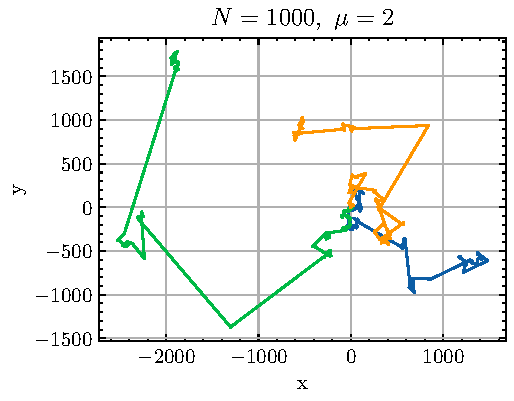
\includegraphics[width=\linewidth]{graphs/N=1000mu=2.pdf}
    
  \end{minipage}%
  \hfill%
  \begin{minipage}{0.48\textwidth}
    \centering
    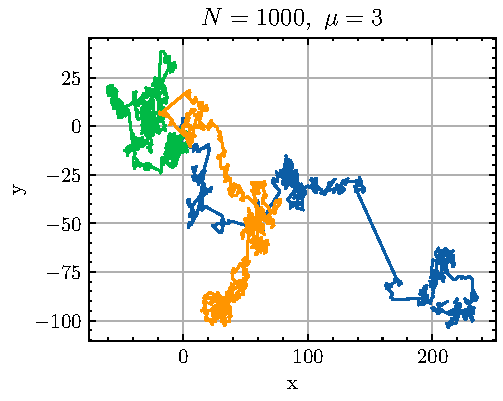
\includegraphics[width=\linewidth]{graphs/N=1000mu=3.pdf}
    
  \end{minipage}

  \begin{minipage}{0.48\textwidth}
    \centering
    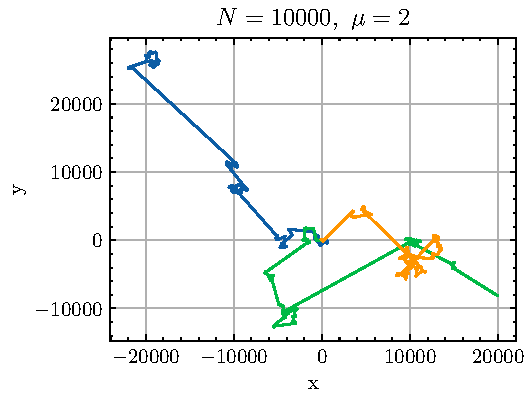
\includegraphics[width=\linewidth]{graphs/N=10000mu=2.pdf}
    
  \end{minipage}%
  \hfill%
  \begin{minipage}{0.48\textwidth}
    \centering
    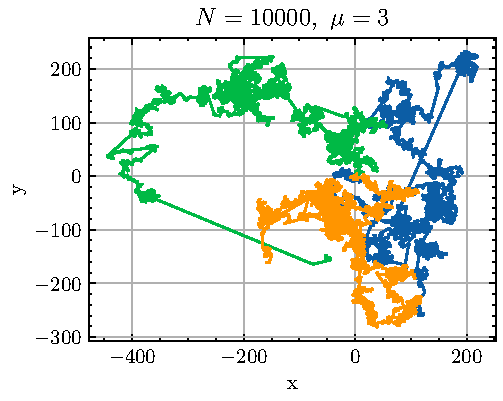
\includegraphics[width=\linewidth]{graphs/N=10000mu=3.pdf}
    
  \end{minipage}
  \caption{3 različni sprehodi za različno število korakov in različen parameter $\mu$}
  \label{fig: sprehodi}
\end{figure}

Iz slike \ref{fig: sprehodi} takoj opazimo, da parameter $\mu$ močno vpliva na obnašanje sprehodov, že sama skala na grafih mora biti dva velikostna reda večja pri $\mu = 2$ da cel sprehod sploh lahko predstavimo. Kasneje bomo videli, da je temu tako ker sta $\mu = 2$ in $\mu = 3$ v različnih režimih, tako kot smo to napovedali že v uvodu.

\subsection{Določanje režimov}

V katerem režimu se nahajamo nam bo povedal faktor $\gamma$ opisan v uvodu. Le tega določimo z linearno regresijo:

$$
  2 * \ln \sigma = \gamma \ln t + c
$$

Za izvajanje regresije sem uporabil $numpy.polyfit$ funkcijo, ki poleg parametrov \textit{fita} določi tudi njihovo napako.

\begin{figure}[ht]
\begin{center}
  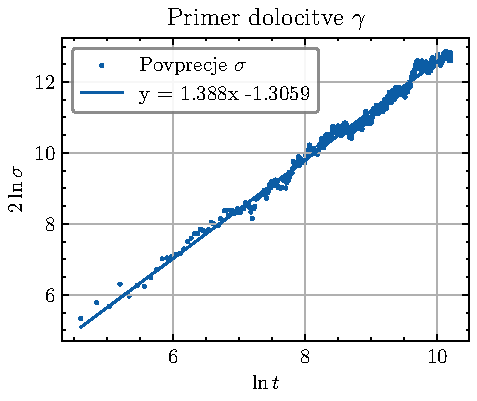
\includegraphics[width=8cm]{graphs/Primerdolocitvegamma.pdf}
  \caption{Faktor $\gamma$ določimo z linearno regresijo. Na sliki je primer regresije za sprehod s parametrom $\mu = 2.5$, z 10 000 koraki in 100 različnimi sprehodi}
  \label{fig: dol_gamma}
\end{center}
\end{figure}

Regresijo ponovimo za nekaj različnih $\mu$ tako za naključne sprehode kot tudi za naključne polete in na ta način dobimo grafe odvisnosti $\gamma$ od $\mu$. Najprej to naredimo za naključne polete, kjer najprej teoretično odvisnost opisano v odvodu lineariziramo in tako na graf \ref{fig: poleti} namesto $\gamma$ rišemo $\gamma^{-1}$

\begin{figure}[ht]
\begin{center}
  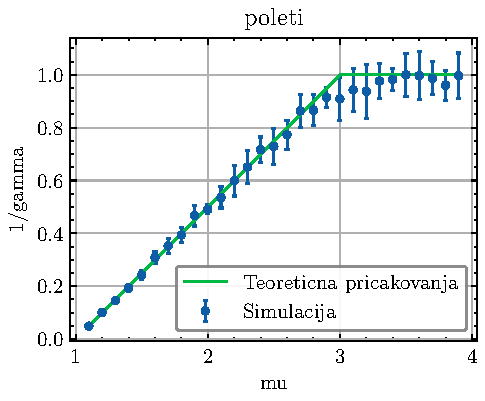
\includegraphics[width=8cm]{graphs/poleti.pdf}
  \caption{$\gamma^{-1}$ v odvisnosti od $\mu$ (20 vzorcev z 100 sprehodi z 10 000 koraki). Skoraj vse simulacije se v intervalu napake skladajo s teoretičnimi napovedmi.}
  \label{fig: poleti}
\end{center}
\end{figure}
\bigskip
Že pri poletih vidimo, da teorija deluje, saj se praktično vsi podatki simulacij skladajo s teorijo v okviru napake. Kljub temu lahko opazimo trend, da okoli točke $\mu = 3$ simulacije najbolj odstopajo. Čeprav nam to morda ni všeč je lahko pojasniljivo. Tam namreč pride do faznega prehoda med super difuzivnim režimom ($\mu < 3$) in normalno difuzijo ($\mu > 3$). Ker simulacija lahko poteka zgolj s končnim številom sprehodov s končnimi koraki, bo seveda ta prehod manj oster.

\bigskip
Vajo ponovimo tudi z naključnimi sprehodi. Te so nekoliko bolj kompleksni za generirati in obdelati, saj časovni intervali med posameznimi koraki niso konstantni, pač pa so sorazmerni z dolžino posameznega koraka. Ker si seveda želimo primerjati mnogo različnih sprehodov ob enakomerno razmaknjenih časih, moramo pozicije ob teh v naprej določenih časih interpolirati iz časa pred in po določenem času. Na srečo za to že obstaja funkcija $np.interp$, saj če bi interpolacije implementirali v pythonu bi nam samo ta operacija vzela cel dan.

Ko pa je ta problem razrešen, je zgodba enaka kot pri naključnih poletih, s to izjemo, da nam ni treba obračati $\gamma$ faktorja. Odvisnost vidimo na grafu \ref{fig: spre}

\newpage
\begin{figure}[ht]
\begin{center}
  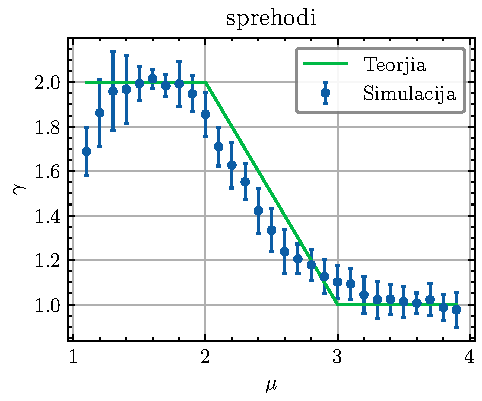
\includegraphics[width=8cm]{graphs/sprehodi.pdf}
  \caption{$\gamma$ v odvisnosti od $\mu$ (20 vzorcev z 100 sprehodi z 10 000 koraki). Simulacije so skoraj v okviru napake. Največje odstopanje opazimo pri $\mu$ blizu 1 in v režimu $2<\mu<3$}
  \label{fig: spre}
\end{center}
\end{figure}

Tudi pri sprehodih opazimo, da teorija deluje precej dobro. Imamo sicer nekoliko manjše ujemanje med simulacijami in teorijo, a vseeno lahko precej dobro ločimo med tremi režimi: pri $\mu<2$ (balistični difuziji) je ujemanje zelo dobro razen pri $\mu$ blizu 1. Ugibam, da imamo na tisti točki nekaj problemov z generacijo naključnih dolžin korakov.



\newpage
\bibliographystyle{plain}
\bibliography{references}


\end{document}